\documentclass[UTF8]{ctexart}
\usepackage{amsmath}
\usepackage{graphicx}
\usepackage{float}
\usepackage{amssymb}
\usepackage{txfonts} 
\usepackage{physics}
\usepackage{float}
\usepackage{tikz}
\newcommand*{\circled}[1]{\lower.7ex\hbox{\tikz\draw (0pt, 0pt)%
		circle (.5em) node {\makebox[1em][c]{\small #1}};}}
\author{1900011413 吴熙楠}
\title{理论力学第二次作业}
\begin{document}
    \maketitle
1.\\
(a)\\
第一宇宙速度$ v_{1}=\sqrt{\frac{GM_{e}}{R_{e}}},v=\frac{1}{2}\sqrt{\frac{GM_{e}}{R_{e}}}\\
E=\frac{1}{2}mv^{2}-\frac{GM_{e}m}{R_{e}}=-\frac{7GM_{e}m}{8R_{e}},L=\frac{m}{4}\sqrt{2GM_{e}R_{e}}\\
m\ddot{r}=-\frac{GM_{e}m}{r^{2}}+\frac{L^{2}}{mr^{3}}\\
 $令$ u=\frac{1}{r},\dot{\theta}=\frac{Lu^{2}}{m}\\
  $代入方程可得:$ \frac{d^{2}u}{d\theta^{2}}+u=\frac{GM_{e}m^{2}}{L^{2}} $\\
  代入数据可得:$  \frac{d^{2}u}{d\theta^{2}}+u=\frac{8}{R_{e}}\\
  u=Acos\theta+Bsin\theta+\frac{8}{R_{e}} $\\
  带入初始条件可得:$ A=-\frac{7}{R_{e}},B=-\frac{1}{R_{e}}\\
  r=\frac{R_{e}}{8-7cos\theta-sin\theta} \\
  (b)$\\
  轨道半长轴$ a=\frac{1}{2}R(1+0.7)=\frac{17}{20}R,E=-\frac{GM_{s}m}{2a}=-\frac{10GM_{s}m}{17R}\\
   $在地球位置处的速度为$ v_{1} $有能量守恒$ \frac{1}{2}mv_{1}^{2}-\frac{GM_{s}m}{R}=-\frac{GM_{s}m}{2a}=-\frac{10GM_{s}m}{17R} \\
   v_{1}=\sqrt{\frac{14GM_{s}}{17R}}$\\
   相对地球:$ \triangle v=\sqrt{\frac{GM_{s}}{R}}(1-\sqrt{\frac{14}{17}}) $\\
   在地球表面发射速度为$ v_{0},\frac{1}{2}m \triangle v^{2}=\frac{1}{2}mv_{0}^{2}-\frac{GM_{e}m}{R_{e}}\\
   v_{0}=\sqrt{\frac{GM_{s}}{R}(\frac{31}{17}-2\sqrt{\frac{14}{17}})+\frac{2GM_{e}}{R_{e}}} \\
   (c)$\\
   以第三宇宙速度发射星体,脱离地球引力后相对地球速度为$(\sqrt{2}-1)\sqrt{\frac{GM_{s}}{R}} \\
   $所以在太阳系看来相对太阳速度是这速度与地球速度矢量叠加 \\
    同(a)的做法:$\frac{d^{2}u}{d\theta^{2}}+u=\frac{GM_{e}m^{2}}{L^{2}},L=mR\sqrt{\frac{GM_{s}}{R}}\\
    	  $带入初始条件可以解得:$ u=\frac{\sqrt{2}-1}{R}sin\theta+\frac{1}{R}\\
    	  r=\frac{R}{1+(\sqrt{2}-1)sin\theta}\\
 2.\\
 (a)\\
 L=\frac{1}{2}m_{1}\dot{\vec{x_{1}}}^{2}+\frac{1}{2}m_{1}\dot{\vec{x_{1}}}^{2}-k|\vec{x}|^{\beta}\\ $
 引入相对位移和质心位矢后可得:$ L=\frac{1}{2}(m_{1}+m_{2})\dot{\vec{R}}^{2}+\frac{1}{2}\frac{m_{1}m_{2}}{m_{1}+m_{2}}\dot{\vec{x}}^{2}-k|\vec{x}|^{\beta} $则化为单体问题\\
而选择质心系后相对质心速度为0,则拉格朗日函数只与相对位矢$\vec{x} $有关,故可以化为一维问题\\
令系统角动量为J,则有有效势能:$ V_{eff}=kr^{\beta}+\frac{J^{2}}{2mr^{2}} $,约化质量$ m=\frac{m_{1}m_{2}}{m_{1}+m_{2}} \\
(b)\\
 V_{eff}=kr^{\beta}+\frac{J^{2}}{2mr^{2}} $\\
 要使扰动为稳定的,则:$V_{eff}^{''} >0 $且$ V_{eff}^{'}|_{r=r_{0}}=0 $\\
 化简得:$ k\beta(\beta+2)>0 $,由已知:$ k\beta>0\\
 \beta>-2 $且$ k\beta>0\\
 \therefore k>0,\beta>0\quad or\quad k<0,-2<\beta <0\\
 (c)\\
  $代入上式化简可得$ L=\frac{1}{2}m\dot{\eta}^{2}-\frac{1}{2}\beta k(\beta+2)r_{0}^{\beta-2} $\\
  可得$ \omega=\sqrt{\frac{k\beta(\beta+2)r_{0}^{\beta-2}}{m}},\quad $其中m为约化质量\\
  (d)\\
  由题意得:系统圆运动角频率$ \omega_{0}=\sqrt{\frac{k\beta r_{0}^{\beta-2}}{m}} \\
  \frac{\omega}{\omega_{0}}=\sqrt{\beta+2} $\\
  当$\frac{\omega}{\omega_{0}}  $为有理数时轨道闭合\\$ 
  \circled{1}\beta=15/25 $时,$ \frac{\omega}{\omega_{0}} $不为有理数,故轨道不闭合\\
  $ \circled{2}\beta=-2/9 $时,$ \frac{\omega}{\omega_{0}}=4/3 $故轨道闭合$ \\
 $如图:(其中蓝线表示微扰前的圆轨道,黄线表示微扰后的轨道) \begin{figure}[H] 
 	\centering
  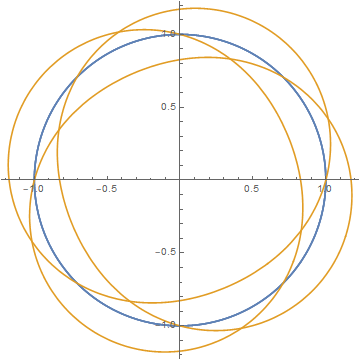
\includegraphics[width=5cm]  {2(d).png}
  \caption{\label{1} 2(d)} 
  \end{figure}$
  3.\\
  $粒子能量为:$E=\frac{1}{2}m\dot{r}^{2}+\frac{J^{2}}{2mr^{2}}+V=1.2V_{0}\\
  J=\sqrt{2mE}s=mr^{2}\dot{\phi}\\
  \phi=\int_{r_{min}}^{\infty}\frac{J/r^{2}}{\sqrt{2m(E-V)-\frac{J^{2}}{r^{2}}}}\,dr\\
  $散射角$\Theta=\pi -2\phi\\
  $微分截面$\frac{d\sigma}{d\Omega}=\frac{sds}{sin\Theta d\Theta}\\
  $其中最近距离满足$:\frac{1}{1+r_{min}}=\frac{6}{5}(1-\frac{s^{2}}{r_{min}^{2}})\\
  $将偏转角度代入进行数值积分可得如图图像$:\\$\begin{figure}[H] 
  	\centering
  	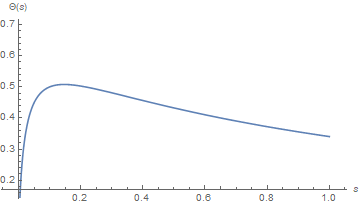
\includegraphics[width=5cm]  {3.1.png}
  	\caption{\label{2} 3.1} 
  \end{figure}
由图2可得:该势能的散射角有最大值,即有最大散射角,大约在s为0.15时取得最大值为0.5\\
将微分截面带入后可得如图:(未标识刻度,其中$\Theta$轴范围为0-0.5,竖直轴范围为0-1,故开始阶段斜率很大)\\
\begin{figure}[H] 
\centering
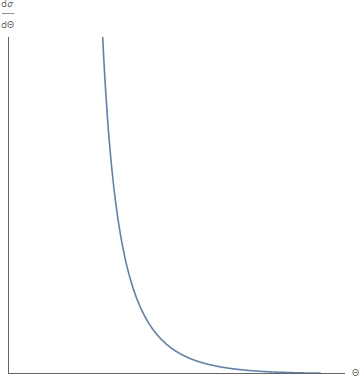
\includegraphics[width=5cm]  {3.2.jpg}
\caption{\label{3} 3.2} 
\end{figure}
我们观察此散射截面曲线可知,在散射角大于0.5时,散射截面降为0,此散射有最大散射角,\\
故由定义有最大散射角的散射会出现彩虹散射可知:会出现彩虹散射\\$
  4.\\
(a)\\
L=\frac{1}{2}m\dot{r}^{2}-\frac{J^{2}}{2mr^{2}}+\alpha\frac{e^{-r/a}}{r} $J为粒子角动量\\
由欧拉拉格朗日方程可得:$ m\ddot{r}=\frac{J^{2}}{mr^{3}}-\alpha(1+\frac{r}{a})\frac{e^{-r/a}}{r^{2}} \\
(b)\\
V_{eff}=\frac{J^{2}}{2mr^{2}}-\alpha\frac{e^{-r/a}}{r}$\\
能量大于0,粒子可以飞向无穷远,能量小于0,则不能飞向无穷远;粒子角动量越大,则粒子的远心点距离越大$ \\
(c)\\V_{eff}=-\frac{\alpha e^{-\frac{r}{a}}}{r}+\frac{J^{2}}{2mr^{2}}\\
$将$V_{eff}$展开到二阶项$:V_{eff}=-\frac{\alpha e^{-\rho/a}}{\rho^{3}}(1+\frac{\rho}{a}+\frac{\rho^{2}}{2a^{2}})r^{2}+\frac{3\alpha(1+\frac{\rho}{a})e^{-\frac{\rho}{a}}}{2\rho^{3}}r^{2}\\
$化简可得:$V_{eff}=\frac{\alpha(1+\frac{\rho}{a}-\frac{\rho^{2}}{a^{2}})e^{-\frac{\rho}{a}}}{2\rho^{3}}r^{2}\\
V_{eff}^{\prime\prime}=\frac{\alpha(1+\frac{\rho}{a}-\frac{\rho^{2}}{a^{2}})e^{-\frac{\rho}{a}}}{\rho^{3}}\\
\omega_{r}=\sqrt{\frac{V_{eff}^{\prime\prime}}{m}}=\sqrt{\frac{\alpha (1+\frac{\rho}{a}-\frac{\rho^{2}}{a^{2}})e^{-\rho/a}}{m\rho^{3}}}
\\$由$m\omega_{0}^{2}\rho=\frac{\alpha e^{-\rho/a}(1+\frac{\rho}{a})}{\rho^{2}}$可得:圆运动角速度为$\omega_{0}=\sqrt{\frac{\alpha (1+\frac{\rho}{a})e^{-\rho/a}}{m\rho^{3}}}\\
\frac{\omega_{r}}{\omega_{0}}=\sqrt{1-\frac{\rho^{2}}{a^{2}+a\rho}}\\$
$\delta \phi=2\pi (1-\sqrt{1-\frac{\rho^{2}}{a^{2}+a\rho}})\\ $
当$a>>\rho$时$,\frac{\omega_{r}}{\omega_{0}}\dot{=}1-\frac{\rho^{2}}{2a^{2}}\\$
故进动角为$:\delta\phi=2\pi\cdot\frac{\rho^{2}}{2a^{2}}=\pi\frac{\rho^{2}}{a^{2}}\\
(d)\\\because$如果保留指数项,将得不出解析解$\therefore$对汤川势展开到一阶$:V=-\frac{\alpha}{r}+\frac{\alpha}{a}\\
$偏转角$\theta=\pi-2\int_{r_{min}}^{\infty}\frac{\frac{J}{r^{2}}}{\sqrt{2m(\frac{1}{2}mv_{\infty}^{2}-\frac{\alpha}{a}+\frac{\alpha}{r})-\frac{J^{2}}{r^{2}}}}\,dr\\$
其中$E=\frac{1}{2}mv_{\infty}^{2},J=mv_{\infty}\rho,d\sigma=\frac{\rho d\rho}{sin\theta d\theta}d\Omega\\$
对比可知:此题只需令$E^{'}=E-\frac{\alpha}{a}$\\即相当于将总能量改变一个常数,此题将等价于卢瑟福散射,但注意角动量不变$\\
$代入卢瑟福散射公式可得散射截面为:$d\sigma=(\frac{\alpha}{2mv_{\infty}^{2}})^{2}\frac{d\Omega}{(1-\frac{2\alpha}{amv_{\infty}^{2}})sin^{4}(\frac{\theta}{2})}$,其中$\Omega$为立体角\\$
5.\\
(a)\\
E_{k}=\frac{1}{2}m(\dot{x_{1}}^{2}+\dot{x_{2}}^{2}),V=\frac{1}{2}k(x_{1}^{2}+x_{2}^{2})+\frac{1}{2}k^{'}(x_{1}-x_{2})^{2},x_{1}\and\ x_{2}$分别为质点偏离平衡的量$ 
M=\begin{pmatrix}
m & 0\\0 & m\end{pmatrix},K=\begin{pmatrix}
	4k&-3k\\-3k&4k\end{pmatrix}\\
	det(M\omega^{2}-K)=0\\
	\omega_{1}=\sqrt{\frac{k}{m}},\omega_{2}=\sqrt{\frac{7k}{m}}\\
(b)\\
$考虑在平衡点列方程可以直接以平衡位置为势能零点,设两物体平衡是距离为l,则:\\
平衡方程为:$\frac{q^{2}}{4\pi\varepsilon_{0}l^{2}}=\frac{3}{2}k(l-l_{0})\\
E_{k}=\frac{1}{2}m(\dot{x_{1}}^{2}+\dot{x_{2}}^{2}),V=\frac{1}{2}k(x_{1}^{2}+x_{2}^{2})+\frac{1}{2}k^{'}(x_{1}-x_{2})^{2}+\frac{q^{2}}{4\pi\varepsilon_{0}(l+x_{2}-x_{1})}$\\
小量近似后并考虑到只有二次项会影响频率\\$ 
V=k(x_{1}^{2}+x_{2}^{2}-x_{1}x_{2})+\frac{q^{2}(x_{1}-x_{2})^{2}}{4\pi\varepsilon_{0}l^{3}}\\
M=\begin{pmatrix}
m & 0\\0 & m\end{pmatrix},K=\begin{pmatrix}
2k+\frac{q^{2}}{2\pi\varepsilon_{0}l^{3}}&-(k+\frac{q^{2}}{2\pi\varepsilon_{0}l^{3}})\\-(k+\frac{q^{2}}{2\pi\varepsilon_{0}l^{3}})&2k+\frac{q^{2}}{2\pi\varepsilon_{0}l^{3}}\end{pmatrix}\\
det(M\omega^{2}-K)=0\\
\omega_{1}=\sqrt{\frac{3k}{m}+\frac{q^{2}}{\pi m\varepsilon_{0}l^{3}}},\omega_{2}=\sqrt{\frac{k}{m}}\\
6.$未给出x方向势能表达式,参考Goldstein前面例题后可知x方向小球质量为mMm,两根弹簧弹性系数均为k,则:$\\
$ 由题目已知的y,z方向势能可知,线性三原子分子在x,y,z方向上的简振模式相同且独立,则以x方向为例:$\\
E_{k}=\frac{1}{2}m_{1}\dot{x_{1}}^{2}+\frac{1}{2}m_{2}\dot{x_{2}}^{2}+\frac{1}{2}m_{3}\dot{x_{3}}^{2}\\
V=\frac{1}{2}k(x_{1}-x_{2})^{2}+\frac{1}{2}k(x_{3}-x_{2})^{2}\\
M=\begin{pmatrix}
m_{1}&0&0\\0&m_{2}&0\\0&0&m_{3}\end{pmatrix},K=\begin{pmatrix}
k&-k&0\\-k&2k&-k\\0&-k&k\end{pmatrix}\\
det(M\omega^{2}-K)=0,m_{1}=m_{3}=m,m_{2}=M\\
\omega_{1}=0,\omega_{2}=\sqrt{\frac{k}{m}},\omega_{3}=\sqrt{\frac{k(M+2m)}{Mm}}\\$
可求出本征矢量:$\eta_{1}=[1,1,1]^{T};\eta_{2}=[1,0,-1]^{T};\eta_{3}=[1,-\frac{2m}{M},1]^{T}\\
q_{1}=x_{1}+x_{2}+x_{3};q_{2}=x_{1}-x_{3};q_{3}=x_{1}-\dfrac{2m}{M}x_{2}+x_{3}\\
$其中,第一种情况对应于分子做匀速直线运动;第二种情况对应于分子中间原子不动,两边原子做对称振动;第三种情况对应于原子相对于分子质心做振动,故可等效为约化质量单原子振动\\
此时只考虑了x方向上的振动,但对比可知y,z方向上和x方向的振动模式相同,故题目得解\\$
7. $\\
在以平衡长度为势能零点时可以抵消重力的影响,假设以板初始位置中心为原点竖直建系,左端点$(-\frac{lcos\phi}{2}+x,y-\frac{l}{2}\phi) $,右端点$(\frac{lcos\phi}{2}+x,y+\frac{l}{2}\phi)$\\
左弹簧$ l_{1}=\sqrt{[x+bsin\theta_{0}+\frac{l}{2}(1-cos\phi)]^{2}+(bcos\theta_{0}-y+\frac{l}{2}\phi)^{2}} $\\右弹簧$ l_{2}=\sqrt{[-x+bsin\theta_{0}+\frac{l}{2}(1-cos\phi)]^{2}+(bcos\theta_{0}-y-\frac{l}{2}\phi)^{2}}\\
E_{k}=\frac{1}{2}m(\dot{x}^{2}+\dot{y}^{2})+\frac{1}{2}\cdot \frac{1}{12}ml^{2}\dot{\phi}^{2}\\
V=\frac{1}{2}k[(l_{1}-b)^{2}+(l_{2}-b)^{2}] $\\
略去高阶项后可得:$ V=\frac{1}{2}k(\frac{l^{2}\phi^{2}cos^{2}\theta_{0}}{2}+2x^{2}sin^{2}\theta_{0}+2y^{2}cos^{2}\theta_{0}+2l\phi xsin\theta_{0}cos\theta_{0}) \\
M=\begin{pmatrix}
m&0&0\\0&m&0\\0&0&\frac{ml^{2}}{12}\end{pmatrix},K=\begin{pmatrix}
2ksin^{2}\theta_{0}&0&klsin\theta_{0}cos\theta_{0}\\0&2kcos^{2}\theta_{0}&0\\klsin\theta_{0}cos\theta_{0}&0&\frac{kl^{2}cos^{2}\theta_{0}}{2}\end{pmatrix}\\
det(M\omega^{2}-K)=0\\
\omega_{1}=\sqrt{\frac{2k}{m}}cos\theta_{0},\omega_{2}=0,\omega_{3}=\sqrt{\frac{k}{m}\cdot(2+4cos^{2}\theta_{0})}\\
$以$x,y,l\phi$为坐标,对于第一种情况,本征矢量: $\eta_{1}=[0,1,0]^{T}\qquad$同理\\$\eta_{2}=[cos\theta_{0},0,-2sin\theta_{0}]^{T},\eta_{3}=[sin\theta_{0},0,6cos\theta_{0}]^{T}\\
$模态矩阵为:$A=\frac{1}{\sqrt{m(1+2cos^{2}\theta_{0})}}$$\begin{pmatrix}
0&\sqrt{3}cos\theta_{0}&sin\theta_{0}\\\sqrt{(1+2cos^{2}\theta_{0})}&0&0\\0&-2\sqrt{3}sin\theta_{0}&6cos\theta_{0}\end{pmatrix}$\\(其中以$l \phi $为第三个坐标)$\\
A^{-1}=\frac{1}{\sqrt{14(1+2cos^{2}\theta_{0})}}$$\begin{pmatrix}
0&\sqrt{(1+cos^{2}\theta_{0})}&0\\\sqrt{3}cos\theta_{0}&0&-2\sqrt{3}sin\theta_{0}\\sin\theta_{0}&0&6cos\theta_{0}\end{pmatrix}\\
Q^{T}=A^{-1}\cdot X\\$故可得简振模式为:$
q_{1}=y;q_{2}=cos\theta_{0}x-2sin\theta_{0}l\phi;q_{3}=sin\theta_{0}x+6cos\theta_{0}l\phi\\
8.\\
(a)\\
X(t)=R\theta(t),x=X(t)+\frac{R}{2}sin\phi,y=R-\frac{R}{2}cos\phi\\
(b)\\
\dot{X}=R\dot{\theta},\dot(x)=R\dot{\theta}+\frac{R}{2}cos\phi\dot{\phi},\dot{y}=\frac{R}{2}sin\phi\dot{\phi}\\
(c)\\
$平动 $ E_{k1}=\frac{1}{2}MR^{2}\dot{\theta}^{2},$转动 $E_{k2}=\frac{1}{2}MR^{2}\dot{\theta}^{2}\\
(d)\\
E_{k3}=\frac{1}{8}mR^{2}(4\dot{\theta}^{2}+\dot{\phi}^{2}+4cos\phi\dot{\phi}\dot{\theta})\\
(e)\\
$由纯滚动条件:$R\dot{\theta}=-\frac{R}{2}\dot{\phi}+\omega \frac{R}{2}$得到$\omega=\dot{\phi}+2\dot{\theta}\\
E_{k4}=\frac{mR^{2}}{16}(\dot{\phi}^{2}+4\dot{\theta}^{2}+4\dot{\phi}\dot{\theta})\\
(f)$\\
取圆筒中心为重力势能零点$V=-\frac{1}{2}mgRcos\phi\\
L=\sum E_{k}-V=MR^{2}\dot{\theta}^{2}+mR^{2}(\frac{3}{4}\dot{\theta}^{2}+\frac{3}{16}\dot{\phi}^{2}+\frac{1}{2}cos\phi\dot{\phi}\dot{\theta}+\frac{1}{4}\dot{\phi}\dot{\theta})+\frac{1}{2}mgRcos\phi\\
(g)\\
\frac{\partial L}{\partial\dot{\theta}}=2MR^{2}\dot{\theta}+mR^{2}(\frac{3}{2}\dot{\theta}+\frac{1}{2}cos\phi\dot{\phi}+\frac{1}{4}\dot{\phi})\\
\frac{\partial L}{\partial\dot{\phi}}=mR^{2}(\dfrac{3}{8}\dot{\phi}+\dfrac{1}{2}cos\phi\dot{\theta}+\dfrac{1}{4}\dot{\theta})\\$
由欧拉拉格朗日方程可以导出:$ \begin{cases} (\frac{4M}{m}+3)\ddot{\theta}+\frac{1}{2}(1+2cos\phi)\ddot{\phi}=sin\phi\dot{\phi}^{2}\\
\frac{1}{2}(1+2cos\phi)\ddot{\theta}+\frac{3}{4}\ddot{\phi}=-\frac{g}{R}sin\phi   \end{cases}\\
(h)\phi<<1$时$,sin\phi\dot{=}\phi,cos\phi\dot{=}1$略去高阶小量后:$
\begin{cases} (\frac{4M}{m}+3)\ddot{\theta}+\frac{3}{2}\ddot{\phi}=0\\
\frac{3}{2}\ddot{\theta}+\frac{3}{4}\ddot{\phi}+\frac{g}{R}\phi=0   \end{cases}$\\
令$\theta,\phi \propto e^{i\omega t}$,则:$
\begin{cases} (\frac{4M}{m}+3)\theta+\frac{3}{2}\phi=0\\
-\frac{3}{2}\omega^{2}\theta+(-\frac{3}{4}\omega^{2}+\frac{g}{R})\phi=0   \end{cases}$\\
方程有非零解的条件为:$(\frac{4M}{m}+3)(-\frac{3}{4}\omega^{2}+\frac{g}{R})+\frac{9}{4}\omega^{2}=0$\\
解之得:$\omega=\sqrt{\frac{g}{R}\cdot\frac{4M+3m}{3M}}$
   \end{document} 